\subsection{Definition}

\subsection{Probabilistic Ontology}

\begin{frame}
	An ontology is an explicit, formal knowledge representation that express knowledge about a domain of application. This includes:
	\begin{itemize}
		\item Types of entities that exist in the domain
		\item Properties of those entities
		\item Relationships among entities
		\item Processes and events that happen with those entities
	\end{itemize}
\end{frame}

\begin{frame}
	A \alert{probabilistic} ontology is an explicit, formal knowledge representation that express knowledge about a domain of application. This includes:
	\begin{itemize}
		\item Types of entities that exist in the domain
		\item Properties of those entities
		\item Relationships among entities
		\item Processes and events that happen with those entities
		\alert{
		\item Statistical regularities that characterize the domain
		\item Inconclusive, ambiguous, incomplete, unreliable, and dissonant knowledge related to entities of the domain
		\item Uncertainty about all the above forms of knowledge
		}
	\end{itemize}
\end{frame}

\begin{comment}
\begin{frame}
	\centering{\LARGE{How to represent \alert{probabilistic} ontologies?}}
	\pause
	\begin{block}{Probabilistic Web Ontology Language (PR-OWL)}
		\begin{itemize}
			\item Created at 2004
			\item Developed by the W3C
			\item As a language to represent ontologies for the Semantic Web
		\end{itemize}
	\end{block}
\end{frame}

\begin{frame}
	\begin{figure}
		\centering
		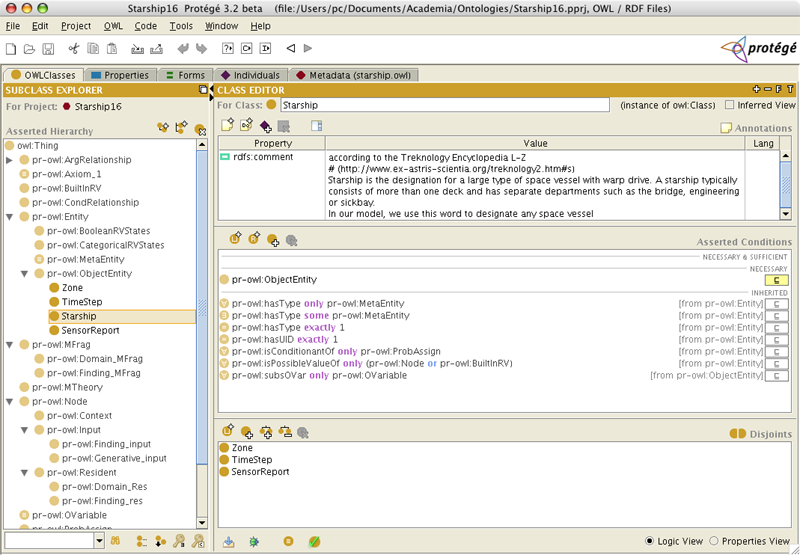
\includegraphics[width=\textwidth]{images/ontology_example}
		\caption{Protegé program}
	\end{figure}
\end{frame}
\end{comment}